\def\Ponderation{45}
\def\SigleNumero{STT-1900}
\def\NomCours{Méthodes statistiques pour ingénieurs}
\def\DateEvaluation{29 février 2024}
\def\HeureEvaluation{18h30 à 21h20}
\def\Session{}
\def\NomEvaluation{Examen 1}

% Ne rien mettre entre les accolades si l'enseignant (ou l'enseignante) est aussi le coordonnateur (ou la coordonnatrice)
\def\Coordonnatrice{}
\def\Coordonnateur{}

% Ne rien mettre entre les accolades s'il y a plus d'une section
\def\Enseignant{}
\def\Enseignante{}

% Ne rien mettre entre les accolades s'il s'agit d'un cours à section unique
% Mettre le nom de chacun des enseignants et enseignantes entre les accolades
% Une case à cocher sera générée pour chacune des sections
\def\SectionA{Ting-Huei Chen}
\def\SectionB{Julien Miron}
\def\SectionC{}
\def\SectionD{}


\def\Directives{
\begin{enumerate}
\item Matériel autorisé:
\begin{itemize}
    \item Calculatrice scientifique {\bf autorisée par la faculté des sciences et de génie};
    \item Une seule feuille aide-mémoire \textbf{manuscrite} de format lettre (8.5''$\times$11'') recto-verso;
    \item Les tables de lois distribuées avec cet examen. S'il-vous-plaît, ne rien écrire sur celles-ci.
    \end{itemize}
\item Assurez-vous que cette évaluation comporte \numquestions ~questions réparties sur \numpages{}~pages, pour un total de \numpoints{}~points.\
\item \textbf{Veuillez ne pas dégrafer votre examen.}
\item Ajoutez vos initiales dans le bas de chaque page (sauf pour les tables de lois).
\item Vous devez\textbf{ justifier toutes vos réponses} par une démarche claire, sauf pour les questions à choix de réponse.\
\item Pour les questions à choix de réponse et les vrais ou faux, vous pouvez mettre un X, un crochet ($\checkmark$) ou remplir la case.\
\item Certains vrais ou faux demande une justification. Aucun point ne sera donné sans justification, même si vous cochez la bonne réponse.
\item Pour les questions à choix de réponse, lorsqu'il est écrit «cochez tous les énoncés qui sont vrais/faux», il est possible qu'un seul énoncé soit vrai.
\item Le verso des feuilles peut être utilisé comme brouillon, \textbf{mais ne sera pas corrigé}. Attention à ne rien dégrafer.
\end{enumerate}
}



\documentclass{Evaluation}
\usepackage{multicol,graphicx}
\begin{document}

\newpage
%%%%%%%%%%%%%%%% QUESTION %%%%%%%%%%%%%%%%
\begin{questions}

\question\label{module1_1}  
On nous donne les probabilités suivantes:
\[
\begin{aligned}
    & P(A) = 0,45 \\
    & P(B) = 0,25 \\
    & P(C) = 0,30 \\
    & P(C|A) = 0,30 \\
    & P(C|B) = 0,30 \\
    & P(A \cap B) = 0,05 \\
\end{aligned}
\]

\begin{parts}
\part[3] Cochez tous les énoncés qui sont \textbf{vrais}.
\begin{checkboxes}
\correctchoice La probabilité de l'événement complémentaire de \(A\), $ P(\overline{A}) = 0,55 $
\choice $P(A \cup B) = 0,70$
\correctchoice $ P(A \cap \overline{B}) = 0,40 $
\choice $ P(A \cap C) = 0,1575 $
\choice $ P(A \cup C) = 0,75 $
\vspace{0.1cm}
\end{checkboxes}

\vspace{0,5cm}

\part[4] \(A\) et \(B\) sont indépendants.

     \begin{oneparcheckboxes}
		\choice VRAI
		\correctchoice FAUX
\end{oneparcheckboxes}\\
{\bf Justification:}
\vspace{4cm}
\end{parts}




\begin{solution}
\begin{parts}
\part
1. $ P(\overline{A}) = 0,55 $\\
2. \(P(A \cup B) = P(A) + P(B) - P(A \cap B)= 0,45 + 0,25 - 0,05 = 0.65 \)\\
3. $ P(A \cap \overline{B}) =  P(A) - P(A \cap B) = 0,45 - 0,05 = 0,40. $\\
4. $ P(A \cap C) = P(A) \cdot  P(C|A) = 0,135 $\\
5. $ P(A \cup C) =  0,45 + 0,3 - 0,135 = 0,615$\\

\part 
FAUX,  \(P(A \cap B) \neq P(A) \cdot P(B)\), 
\( P(A \cap B) = 0,45 \cdot 0,25 \).\\


\end{parts}
\end{solution}

\question[3]\label{normaleBivariee}
La résistance au cisaillement $Y$ et le diamètre $X$ de soudures par points ont fait l'objet d'une étude visant à remplacer un essai destructif par un essai non destructif. Voici les conclusions de cette étude.
\begin{enumerate}
    \item Le vecteur $[X,Y]$ obéit à une loi normale bivariée.
    \item $\mu_X=0,20$ cm, $\mu_Y=1100$ kg, $\sigma^2_X=0,02$ cm$^2$, $\sigma^2_Y=525$ kg$^2$ et $\rho = 0,9$.
\end{enumerate}

En supposant que le diamètre vaut $d$ cm, quelle est l'expression de l'espérance de $Y$, sachant que $X=d$?

 \begin{checkboxes}
		\choice $E[Y|X=d]=1100$  %  X1
		\correctchoice $E[Y|X=d]=145,8d + 1070,84$ kg % X_2 | X1
		\choice $E[Y|X=d]=1100,20$ kg % X_2 
		\choice $E[Y|X=d]=1100+d$ kg% X_1 | X2
		\choice $E[Y|X=d]=145,8d + 1100$ kg% X_2 | X1 avec sigma^2 plutot que sigma
\end{checkboxes}

\vspace{0.5cm}

\question[3] Soit $K$, $S$ et $F$ des variables aléatoires indépendantes qui suivent respectivement une khi-carré à 4 degrés de liberté, une Student à 35 degrés de liberté et une Fisher à 3 et 4 degrés de liberté. 

Cochez tous les énoncés qui sont \textbf{faux}?

\begin{checkboxes}
		\correctchoice $P(S>35)=0,50$
		\choice $P(K<9,49)=0,95$
		\choice $P(F>6,59)=0,05$
		\choice $P(S>a \cap K> b \cap F >c)= P(S>a)\times P(K>b)\times P(F>c)$
\end{checkboxes}

\newpage
\question[6]\label{module1_2} 
Dans une usine, deux machines, A et B, produisent des composants. La machine A produit 45\% des composants et la machine B produit le reste. 15\% des composants produits par A sont défectueux, tandis que 10\% des composants produits par B sont défectueux. Si un composant est défectueux, quelle est la probabilité qu'il ait été produit par la machine A?

\begin{solution}
Soit \( D \) l'événement qu'un composant soit défectueux et \( A \) l'événement qu'il ait été produit par la machine A.

Nous cherchons \( P(A|D) \), la probabilité que le composant ait été produit par la machine A sachant qu'il est défectueux.

Par la formule de Bayes:
\[ P(A|D) = \frac{P(D|A) \cdot P(A)}{P(D)} \]

Les données fournies sont:
\[ P(A) = 0,45 \]
\[ P(B) = 0,55 \]
\[ P(D|A) = 0,15 \]
\[ P(D|B) = 0,10 \]

Calculons \( P(D) \) en utilisant la loi des probabilités totales:
\[ P(D) = P(D|A) \cdot P(A) + P(D|B) \cdot P(B) = 0,1225 \]

Maintenant, nous pouvons substituer ces valeurs dans la formule de Bayes:
\[ P(A|D) = \frac{0,45 \cdot 0,15}{0,1225} = 0.551 \]
\end{solution}

\vfill

\question[10]
Déterminez si les énoncés suivants sont vrais ou faux. 

\textbf{\textit{Une bonne réponse vaut 2 points, une mauvaise réponse vaut -1 point et une réponse vide vaut 0 point, pour un total minimum de 0 point.}}

\begin{parts}
    \part Si $X_1,\hdots,X_{100}$ constituent un échantillon aléatoire simple issu d'une loi quelconque d'espérance $\mu=0$ et d'écart-type $\sigma=10$, alors la moyenne échantillonnale de ces 100 valeurs suit approximativement une loi normale centrée-réduite. 

    \begin{oneparcheckboxes}
        \choice Vrai
        \correctchoice Faux
    \end{oneparcheckboxes}

    \begin{solution}
        Faux
    \end{solution}
    \vspace{0.5cm}
    \part Si $X_1,\hdots,X_{17}$ constituent un échantillon aléatoire simple issu d'une loi $\mathcal{N}(5; 4)$, alors la variable $16S^2$ a une espérance de 16 et une variance de 32. 

    \begin{oneparcheckboxes}
        \correctchoice Vrai
        \choice Faux
    \end{oneparcheckboxes}
        \begin{solution}
        Vrai
    \end{solution}
        \vspace{0.5cm}

    \part Si $W$ suit une $\chi^2_4$ (khi-carré avec $4$ degrés de liberté), alors la densité de $W$ est symétrique. 

    \begin{oneparcheckboxes}
        \choice Vrai
        \correctchoice Faux
    \end{oneparcheckboxes}
    
    \begin{solution}
        Faux
    \end{solution}
        \vspace{0.5cm}
    \item Le poids des tomates d'un certain agriculteur suit une loi normale de moyenne $300\text{ grammes}$ et de variance $100\text{ grammes}^2$. On prend des mesures sur 25 tomates choisies aléatoirement et on obtient une moyenne échantillonnale de $309,12\text{ grammes}$ et une variance échantillonnale de $118,3\text{ grammes}^2$. Dans cette situation, les nombres $309,12$ et $118,3$ sont des paramètres et les nombres $300$ et $100$ sont des statistiques.
    
    \begin{oneparcheckboxes}
        \correctchoice Vrai
        \choice Faux
    \end{oneparcheckboxes}
            \begin{solution}
        Vrai
    \end{solution}
        \vspace{0.5cm}


    \part Soit deux échantillons aléatoires indépendants de taille $n_1=26$ et $n_2=26$ qui proviennent de lois normales $\mathcal{N}(\mu_1, \sigma^2)$ et $\mathcal{N}(\mu_2, \sigma^2)$. Les moyennes échantillonnales sont respectivement $\overline{X}_1$ et $\overline{X}_2$, alors que les variances échantillonnales sont respectivement $S^2_1$ et $S^2_2$. La statistique $S^2_1/S^2_2$ suit une $F_{25,25}$. 

    \begin{oneparcheckboxes}
        \correctchoice Vrai
        \choice Faux
    \end{oneparcheckboxes}
    
            \begin{solution}
        Vrai
    \end{solution}

    \end{parts}
    \newpage
\newpage
\question \label{module2}
$X$ est une variable aléatoire continue dont la densité est donnée par:
\[ f(x) =
\begin{cases}
   \displaystyle\frac{6}{5}(1 - 2x^2) & \text{si } -0.5 < x < 0.5 \\
    0 & \text{sinon}.
\end{cases}
\]


\begin{parts}
\part[3] Cochez tous les énoncés qui sont \textbf{vrais}.
\begin{checkboxes}
\correctchoice $F(x)=\displaystyle\frac{6}{5}(x - \frac{2}{3}x^3 + \frac{5}{12} )$ 
\correctchoice \(E(3X + 20) = 3 E(X)\)
\choice \(V(2X) = 2 V(X) \)
\choice \(V(X + 10)  > V(X)\)
\vspace{0.1cm}
\end{checkboxes}


\vspace{0,5cm}

\part[4] \(V(X) = E(X^2) - 2E(X)^2\).

     \begin{oneparcheckboxes}
		\choice VRAI
		\correctchoice FAUX
\end{oneparcheckboxes}\\
{\bf Justification:}
\vspace{4cm}

\part[6] Calculez \(P( X < 0  \mid X > -0.25)\):

\end{parts}


\begin{solution}
\begin{parts}
\part 
0. Calcul de la valeur de \(k\):\\

L'intégrale de la densité sur toute la plage doit être égale à 1 :
\[ \int_{-0.5}^{0.5} k(1 - 2x^2) \,dx = 1 \]

Calculons cette intégrale :
\[ \int_{-0.5}^{0.5} k(1 - 2x^2) \,dx = \frac{5k}{6} \]

Pour que l'intégrale soit égale à 1, la constante \(k\) doit être \(\frac{6}{5}\).\\

1. Obtention de la fonction de répartition de \(X\):\\

La fonction de répartition \(F(x)\) est obtenue en intégrant la densité \(f(x)\) de moins l'infini à \(x\):
\[ F(x) = \int_{-0.5}^{x} f(t) \,dt =
k \left\{ \left(x - \frac{2}{3}x^3\right) - \left(-0.5 - \frac{2}{3}(-0.5)^3\right) \right\} =
k \left\{x - \frac{2}{3}x^3 + \frac{5}{12}   \right\} 
\]

2. \(E(3X + 20) = 3 E(X) + 20\)\\
3. \(V(2X) = 4 V(X) \) \\
4. \(V(X + 10)  = V(X)\)


\part 
FAUX,  5. \(V(X) = E(X^2) - E(X)^2\)\\ 

\part  Calcul de \(P(X < 0 \mid X > -0.25)\):

\[ P(X < 0 \mid X > -0.25) = \frac{P(X < 0 \cap X > -0.25)}{P(X > -0.25)}  = (0.5 - 0.2125)/0.7875 = 0.365\]

\end{parts}
\end{solution}


\newpage
\question\label{module3} 
Supposons qu'un ingénieur travaille sur le développement de deux capteurs de température pour un processus industriel. On peut modéliser les mesures des deux capteurs $X$ et $Y$ comme deux variables aléatoires normales indépendantes, avec des moyennes respectives \( \mu_X = 20 \) et \( \mu_Y = 25 \) et des variances \( \sigma_X^2 = 4 \) et \( \sigma_Y^2 =9\).\\

\begin{parts}
\part[3] Cochez tous les énoncés qui sont \textbf{vrais}.
\begin{checkboxes}
\correctchoice $X - Y$ est également une variable aléatoire qui suit une loi normale.
\choice $\displaystyle \frac{X-20}{4}\sim \mathcal{N}(0, 1)$
\choice \(P(X < 18.5) > P(X > 21.5)\).
\choice  \(P(Y < 20) > P(Y > 29)\).
\vspace{0.1cm}
\choice  \(P(X < 18) < P(Y < 18)\)
\end{checkboxes}

\vspace{0,5cm}

\part[4] $\text{Var}\left[X - Y\right]< \text{Var}\left[X + Y\right]$.

     \begin{oneparcheckboxes}
		\choice VRAI
		\correctchoice FAUX
\end{oneparcheckboxes}\\
{\bf Justification:}
\vspace{5cm}

%\part Quelle est la valeur, disons \(v\), telle que 2,5\% des mesures de \(X\) représentent une température inférieure à \(v\) ?\\
\part[6] Calculez $P(5Y > 4X + 62)$.

\end{parts}

\begin{solution}
\begin{parts}
\part 
1. Oui.\\
2. $\frac{X-20}{2}\sim \mathcal{N}(0, 1)$\\
3.  \(P(X < 18.5) = P(X > 21.5)\).\\
4. \(P(Y < 20) < P(Y > 29)\).\\
5.  \(P(X < 18) > P(Y < 18)\)\\

\part 
FAUX,  $\text{Var}\left[X - Y\right] =  \text{Var}\left[X + Y\right]$\\

\part
%$F(\frac{v - 20}{2}  ) = \Phi(z)  = 0,025$. Donc, $\frac{v - 20}{2} = -1,96$, $v = 16,08$


$P(5Y > 4X + 62) = P(5Y - 4X > 62)$


Les moyennes et variances des variables \(X\) et \(Y\) sont utilisées pour déterminer la moyenne \(\mu_W\) et la variance \(\sigma_W^2\) de la variable aléatoire \(W = 5Y - 4X\). 

\[
\begin{align*}
\mu_W &=  5\mu_Y - 4\mu_X  = 5 \times 25 - 4 \times 20   = 45 \\
\sigma_W^2 &= 25\sigma_Y^2 + 16\sigma_X^2 = 25 \times 9 + 16 \times 4 =  225 + 64 = 289 \\
P(5Y  - 4X  > 62) &= P(Z > \frac{62- 45}{17}) \\
&= 1 - \Phi(1) = 0,15866
\end{align*}
\]


\end{parts}
\end{solution}


\newpage



\question\label{conjointe}

Soit $X$ et $Y$ deux variables aléatoires dont la loi conjointe est 
$$f(x,y)=\left\{
			\begin{array}{ll}
   \displaystyle \frac{e^{-x}}{b-a}  & \mbox{ si } 0\leq x \ \mbox{ et } \ a\leq y\leq b, \\
    0  & \mbox{ sinon. }
			\end{array}
			\right.$$

Dans cette fonction de densité, $a<b$. Nous savons que la fonction de densité marginale de $X$ est
$$f_X(x)=\left\{
			\begin{array}{ll}
   \displaystyle e^{-x} & \mbox{ si } 0\leq x ,\\
    0  & \mbox{ sinon. }
			\end{array}
			\right.$$

\begin{parts}
\part[6] Quelle est la fonction de densité marginale de $Y$?


\vspace{15cm}

\part[3] Les variables aléatoires $X$ et $Y$ sont-elles indépendantes?

     \begin{oneparcheckboxes}
		\choice OUI
		\choice NON
\end{oneparcheckboxes}\\
{\bf Justification:}


\vfill

\pagesuivante{\ref{conjointe}}
\newpage
\suite{\ref{conjointe}}
\part[6] Si $a=0$ et $b=1$, calculez $P(X\leq1 \cap Y>0,5)$.


\begin{solution}
\begin{align*}
    P(0\leq X\leq 1) =& \int_{0}^1 f_X(x)dx\\
    =& \int_{0}^1 \frac{1}{2}\exp(-\frac{x}{2})dx\\
    =& \left. -\exp(-\frac{x}{2})\right|_0^1\\
    =& 1-\exp(-1/2)\\
    \approx& 0,3935
    \end{align*}
\end{solution}


\end{parts}

\newpage

\question[]\label{micro}
Dans un laboratoire de microtechnique, Audrey et Vincent ont étudié le temps de réaction (en millisecondes) d'un certain type de détecteur de mouvements. Les 21 valeurs suivantes sont des temps de réaction collectés au cours d'une journée:

\begin{center}
\begin{tabular}{  c c c c c c c c }
111  &111  &111  &112  &113  &113  &113 \\
113 &115  &115  &115  &115 &115 & 116 \\
118 & 118 & 118 & 119 & 125 &125 & 125\\
\end{tabular}
\end{center}

Le diagramme en boîte ci-dessous a été tracé à partir de ces résultats. Il y a toutefois une erreur (il ne s'agit pas d'un titre ou de noms d'axes).

\medskip
\begin{center}
		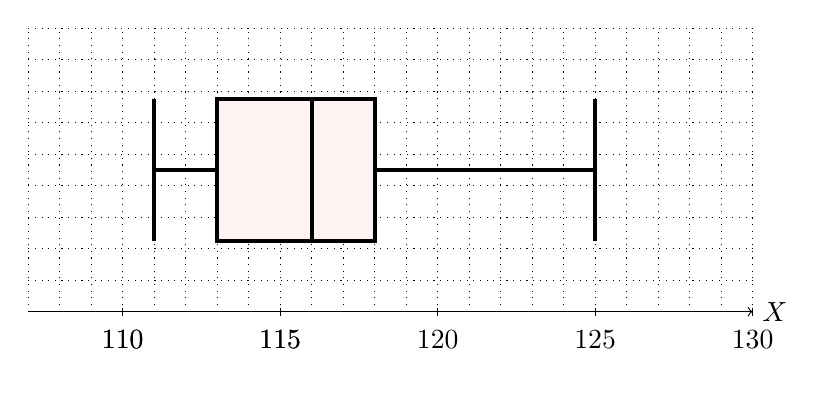
\begin{tikzpicture}[x=0.4cm,y=0.9cm]
         \draw[step=0.4cm,,dotted,color=black] (107,0) grid (130,4);
		\draw[->] (107,0) -- (130,0) node[right] {$X$} ;
		\foreach \X in {110,115,110,115,120,125,130} {
			\draw (\X,0.05cm) -- (\X,-0.05cm) node[below] {$\X\strut$};}
		\draw[ultra thick][fill=red!5] (113,1) rectangle (118,3);
  	\draw[ultra thick] (116,1) -- (116,3);

		\draw[ultra thick] (111,1) -- (111,3);
		\draw[ultra thick] (111,2) -- (113,2);
		\draw[ultra thick] (118,2) -- (125,2);
		%\draw[ultra thick] (4,1) -- (4,3);
		\draw[ultra thick] (125,1) -- (125,3);

			\end{tikzpicture}\\
	\end{center}
\begin{parts}



 \part[3] Quelle est cette erreur?

  \begin{checkboxes}
\choice La médiane n'est pas au bon endroit.  %  X1
\choice La moyenne échantillonnale n'est pas au bon endroit. % X_2 | X1
\choice Il devrait y avoir deux points: un à 105,5 et un à 125,5.
\choice La moustache de gauche devrait être à  105,5 % X_2 
\choice La moustache de droite devrait être à 125,5 % X_1 | X2
\end{checkboxes}

\vspace{1cm}

\part[6] Nous apprenons qu'une observation (125) est erronée. Nous ne connaissons pas sa valeur, mais nous savons que celle-ci est plus grande que 150. Nous notons cette valeur XXX et nous savons que XXX~$>$~150. Le nouveau jeu de données est donc:

\begin{center}
\begin{tabular}{  c c c c c c c c }
111  &111  &111  &112  &113  &113  &113 \\
113 &115  &115  &115  &115 &115 & 116 \\
116 & 118 & 118 & 119 & 125 &125 & XXX\\
\end{tabular}
\end{center}

À partir de ce nouveau jeu de données, répondez aux questions suivantes. Nous nommons «jeu de données original» celui qui contient l'observation 125 et «nouveau jeu de données» celui qui contient l'observation XXX.

Déterminez si les énoncés suivants sont vrais ou faux. 

\textbf{\textit{Une bonne réponse vaut 2 points, une mauvaise réponse vaut -1 point et une réponse vide vaut 0 point, pour un total minimum de 0 point.}}

\begin{subparts}
\subpart La médiane échantillonnale du nouveau jeu de données est supérieure à celle du jeu de données original.

    \begin{oneparcheckboxes}
        \choice Vrai
        \correctchoice Faux
    \end{oneparcheckboxes}
    
\begin{solution}
    Faux
\end{solution}

\subpart La moyenne échantillonnale du nouveau jeu de données est supérieure à celle du jeu de données original.

    \begin{oneparcheckboxes}
        \correctchoice Vrai
        \choice Faux
    \end{oneparcheckboxes}
    
\begin{solution}
    Vrai
\end{solution}

\subpart La variance échantillonnale du nouveau jeu de données est supérieure à celle du jeu de données original.

    \begin{oneparcheckboxes}
        \correctchoice Vrai
        \choice Faux
    \end{oneparcheckboxes}
    
\begin{solution}
    Vrai
\end{solution}

\end{subparts}
\end{parts}

\newpage

\question\label{estimateursPonctuels} 
Soit $X_1$ et $X_2$ deux réalisations d'une variable $X\sim\mathcal{N}(0, 4)$. Nous avons que $X_1$ et $X_2$ sont indépendantes et nous notons

\begin{align*}
    \overline{X}=\displaystyle \frac{X_1+X_2}{2}, & & S^2=\sum_{i=1}^2(X_i-\overline{X})^2.
\end{align*}

\begin{parts}
    \part[7] Calculez $P(\overline{X}>S^2)$. 
    
    \begin{solution}
        \begin{align*}
            P(\overline{X} > \mu + 0,62S)
            &= P(\overline{X} - \mu  > 0,62S) \cr
             &= P\left(\frac{\overline{X} - \mu}{S/\sqrt{n}}  >  \frac{0,62 S}{S/\sqrt{n}}\right) \cr
             &= P\left( T_{n-1} >  0,62 {\sqrt{9}}\right) \cr
             &= P\left( T_{8} > 1,86\right) \cr
             &= 0,05
        \end{align*}
    \end{solution}
\vspace{10cm}
    \part[6] Calculez la probabilité que la variance échantillonnale soit inférieure à 15,36.

    
        \begin{solution}
        \begin{align*}
            P(S^2 > 1,09)
             &= P\left(\frac{(n-1)S^2}{\sigma^2}  > \frac{(n-1)1,09}{\sigma^2}\right) \cr
             &= P\left( \chi_{n-1}^2  > \frac{8\times 1,09}{4}\right) \cr
             &= P\left( \chi_{8}^2  > 2,18 \right) \cr
             &= 0,975
        \end{align*}
    \end{solution}
\end{parts}
\newpage

\question[8]
Un producteur de Vacherin Fribourgeois sait que le poids d'une de ses meules de fromage, $X$, est une variable aléatoire d'espérance $\mu=7$ kg et de variance $\sigma^2 = 1$ kg$^2$. Il doit envoyer 100 meules à un festival. Le transporteur lui chargera 1500\$, à condition que le poids total des 100 meules soit inférieur ou égal à $720$ kg. Dans le cas contraire, il lui chargera 2000\$.

Quelle est la probabilité approximative que le transporteur lui charge 2000\$?
    \vspace{12cm}

\end{questions}

\end{document} 
